\documentclass[aspectratio=169, xcolor=dvipsnames]{beamer}

\usepackage{graphicx}
\usepackage{soul}
\usepackage{textcomp}

% Téma
\usetheme{Luebeck}
\setbeamercolor*{structure}{bg=PineGreen!20,fg=PineGreen}
\setbeamercolor*{palette primary}{use=structure,fg=white,bg=structure.fg}
\setbeamercolor*{palette secondary}{use=structure,fg=white,bg=structure.fg!75}
\setbeamercolor*{palette tertiary}{use=structure,fg=white,bg=structure.fg!50!black}
\setbeamercolor*{palette quaternary}{fg=white,bg=black}
\setbeamercolor{section in toc}{fg=black,bg=white}
\setbeamercolor{alerted text}{use=structure,fg=structure.fg!50!black!80!black}
\setbeamercolor{titlelike}{parent=palette primary,fg=structure.fg!50!black}
\setbeamercolor{frametitle}{bg=gray!10!white,fg=PineGreen}
\setbeamercolor*{titlelike}{parent=palette primary}

% Titulní strana
\title{Semestrální práce}
\subtitle{KIV/PPR}
\author{Jan Hereš}
\date{10.10.2023}

\begin{document}
\begin{frame}
	\titlepage
\end{frame}

\begin{frame}{Osnova}
	\begin{enumerate}
    \item Teoretická část
      \begin{itemize}
        \item Analýza zadání 
        \item Analýza související studie a dostupných dat 
        \item Normalizace dat
        \item Algoritmus pro hledání vzorce korelace
        \item Výpočet korelace dat
      \end{itemize}

    \item Praktická část
      \begin{itemize}
        \item Control a Data flow diagram
        \item Poznámky k řešení
      \end{itemize}
    \item Závěr
  \end{enumerate}
\end{frame}

\begin{frame}
 \begin{center}
    Teoretická část 
 \end{center} 
\end{frame}

\begin{frame}{}
	\begin{center}
\begin{enumerate}
    \item Teoretická část
      \begin{itemize}
        \item Analýza zadání 
       \end{itemize}
   \end{enumerate}
	\end{center}
\end{frame}


\begin{frame}{Teoretická část - Analýza zadání}
	\begin{block}{Analýza zadání}
    \pause
    \begin{itemize} 
      \item \textbf{Cíl}: Najděte vzorec pro \textcolor{Red}{korelaci} mezi akcelerometrem a srdečním tepem
        \pause
      \item K dispozici máte naměřená data (ACC - X,Y,Z a HR - tepové frekvence) $\to$ proveďte jejich \textcolor{Red}{normalizaci}
        \pause
      \item Při hledání vzorce ideálně využijte koncepty \textcolor{Red}{genetického programování} či \textcolor{Red}{gramatické evoluce}  
        \pause
      \item Spočítejte jejich korelaci pomocí vybrané statistické metody \pause $\to$ \textcolor{Red}{fitness funkce}
        \pause
      \item ,,Best-fit'' vygenerovanou funkci zobrazte \textcolor{Red}{v grafu} (SVG)
    \end{itemize}
	\end{block}
\end{frame}

\begin{frame}{}
	\begin{center}
\begin{enumerate}
    \item Teoretická část
      \begin{itemize}
        \item Analýza zadání 
        \item Analýza související studie a dat
       \end{itemize}
   \end{enumerate}
	\end{center}
\end{frame}


\begin{frame}{Teoretická část - Analýza související studie a dat}
	\begin{block}{Analýza studie}
    \pause
		\begin{itemize}
      \item Sledované subjekty \textcolor{Red}{netrpí žádnými kardiovaskulárnimi problémy}
        \pause
        \begin{itemize}
          \item v opačném případě by bylo nutné zavést komplexnější normalizaci dat $\to$ \textcolor{Red}{značné usnadnění práce}
          \item jednodušší vytvoření závěrů (!)
        \end{itemize}
      \pause
      \item Frekvence sběru dat ze senzorů: ACC = \textcolor{Red}{32 Hz}, HR = \textcolor{Red}{1 Hz} 
        \pause
        \begin{itemize}
          \item Je potřeba řešit různost frekvence sběru dat?
            \pause
          \item Pokud budeme počítat klouzavý průměr, není potřeba (dle mého názoru) dalších úprav 
            \begin{itemize}
              \item Jak ale určit správnou sledovanou periodu? 
            \end{itemize}
        \end{itemize}
    \end{itemize}
	\end{block}
\end{frame}

\begin{frame}{Teoretická část - Analýza související studie a dat}
  \begin{block}{Určení společné periody sledování}
    \begin{itemize}
        \pause
      \item Jako první se nabízí sjednotit na periodu 1Hz (1s)
        \pause
      \item Ale má pak smysl pozorovat korelaci v sekundách? 
        \pause
      \item Naopak, neztrácíme informace při moc dlouhé periodě? 
        \pause
      \item Ideální řešení? \pause vyzkoušet \textcolor{Red}{více různých nastavení} (1s, 10s, 30s, 60s)
        \pause
        \begin{itemize}
          \item Zvolená perioda bude \textbf{zásadní} pro správnou prezentaci výsledků!
        \end{itemize}
    \end{itemize} 
  \end{block} 
\end{frame}

\begin{frame}{Teoretická část - Analýza související studie a dat}
  \begin{block}{Pár statistických údajů}
    \begin{itemize}
      \item Největší soubor velikostně do 1,1GB
      \item Rozsah hodnot ACC: \textless-128.0; 127.0\textgreater 
      \item Rozsah hodnot HR: v rámci rozsahu \textless0; 255\textgreater
      \item Tyto údaje budou důležité zejména v \textbf{praktické} části
    \end{itemize} 
  \end{block} 
\end{frame}

\begin{frame}{}
	\begin{center}
\begin{enumerate}
    \item Teoretická část
      \begin{itemize}
        \item Analýza zadání 
        \item Analýza související studie a dat
        \item Normalizace dat
       \end{itemize}
   \end{enumerate}
	\end{center}
\end{frame}


\begin{frame}{Teoretická část - Normalizace dat}
  \begin{block}{Normalizace dat}
    \begin{itemize}
        \pause
      \item Vypočtené klouzavé průměry budou normalizovány na interval (0;1)
        \pause
        \begin{itemize}
          \item $\to$ globální vs lokální normalizace? 
            \pause
          \item Pro tento specifický případ považuji za vhodnější \textcolor{Red}{globální} normalizaci (neočekávám zásadní vliv \textit{outlierů}) 
        \end{itemize}
        \pause
      \item Veličiny akcelerometru (X, Y, Z) budou považovány za 3 samostatné veličiny
        \begin{itemize}
          \item Budou sledovány korelace v jednotlivých směrech pohybu
        \end{itemize}
    \end{itemize} 
  \end{block} 
\end{frame}



\begin{frame}{}
	\begin{center}
\begin{enumerate}
    \item Teoretická část
      \begin{itemize}
        \item Analýza zadání 
        \item Analýza související studie a dat
        \item Normalizace dat
        \item Výpočet korelace dat
       \end{itemize}
   \end{enumerate}
	\end{center}
\end{frame}


\begin{frame}{Teoretická část - Výpočet korelace dat}
  \begin{block}{Možnosti řešení}
    \begin{itemize}
        \pause
       \item Pearson's correlation coefficient
         \pause
        \begin{itemize}
          \item Nejrychlejší řešení, ale principiálně omezen na \textcolor{Red}{lineární} vazbu  
        \end{itemize}
        \pause
      \item Spearman's Rank correlation
        \pause
        \begin{itemize}
          \item Teoreticky lepší řešení
            \pause
          \item Ale vyžaduje řazení dle váhy (hodnoty) - \textcolor{Red}{pomalé}
        \end{itemize}
        \pause
      \item Mutual information
        \begin{itemize}
          \item Obecně nevhodné na tento problém 
        \end{itemize}
      \item Distance correlation
        \begin{itemize}
          \item Teoreticky nejlepší řešení, ale principiálně velmi náročné  
        \end{itemize}
    \end{itemize} 
  \end{block} 
\end{frame}

\begin{frame}{Teoretická část - Výpočet korelace dat}
  \begin{block}{Pearsonův koeficient korelace}
    \begin{itemize}
        \pause
       \item Základní postup
         \begin{center}
           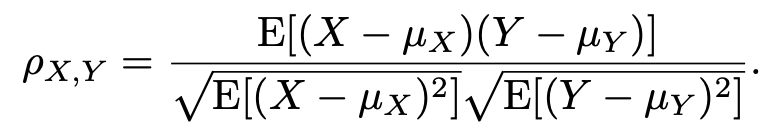
\includegraphics[width=\linewidth]{assets/pearson-twopass.png}; 
         \end{center}
     \end{itemize} 
  \end{block} 
\end{frame}

\begin{frame}{Teoretická část - Výpočet korelace dat}
  \begin{block}{Pearsonův koeficient korelace}
    \begin{itemize}
     \item Alternativně
        \begin{center}
          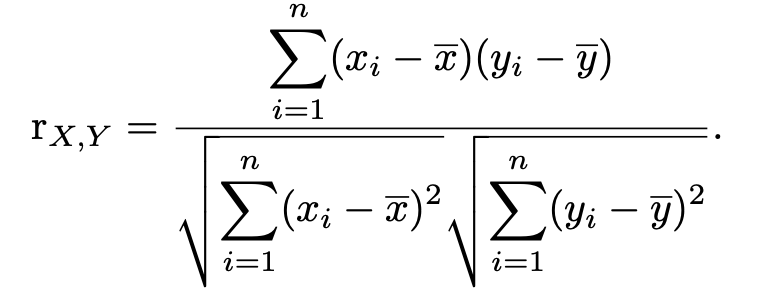
\includegraphics[width=\linewidth]{assets/pearson-twopass-2.png}
        \end{center}
     \end{itemize} 
  \end{block} 
\end{frame}

\begin{frame}{Teoretická část - Výpočet korelace dat}
  \begin{block}{Pearsonův koeficient korelace}
    \begin{itemize}
      \item Základní postup - \textcolor{Red}{Nevýhody}
        \begin{itemize}
          \item Vyžaduje dva prostupy daty
          \item Numericky nestabilní pro velká data 
        \end{itemize}
     \end{itemize} 
  \end{block} 
\end{frame}

\begin{frame}{Teoretická část - Výpočet korelace dat}
  \begin{block}{Pearsonův koeficient korelace}
    \begin{itemize}
      \item Naivní \textit{one-pass} algoritmus
        \begin{center}
          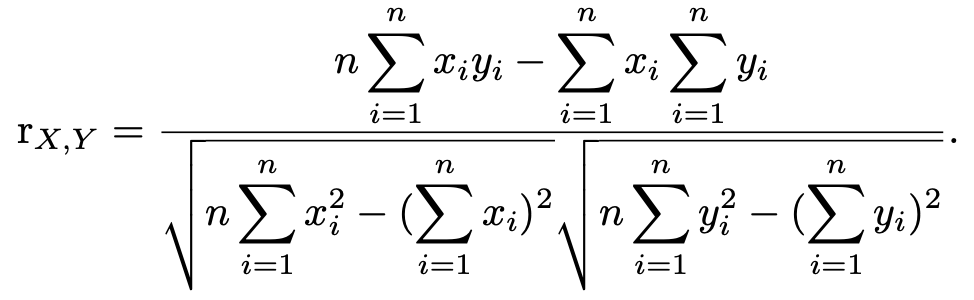
\includegraphics[width=\linewidth]{assets/pearson-onepass-naive.png} 
        \end{center}
     \end{itemize} 
  \end{block} 
\end{frame}

\begin{frame}{Teoretická část - Výpočet korelace dat}
  \begin{block}{Pearsonův koeficient korelace}
    \begin{itemize}
      \item Naivní \textit{one-pass} algoritmus - \textcolor{Red}{Nevýhody}
        \begin{itemize}
          \item Stále numericky nestabilní pro velká data
        \end{itemize}
     \end{itemize} 
  \end{block} 
\end{frame}

\begin{frame}{Teoretická část - Výpočet korelace dat}
  \begin{block}{Pearsonův koeficient korelace}
    \begin{itemize}
      \item Stabilní \textit{one-pass} algoritmus  \\
        $ \bar{x}^{'} = \bar{x} + \frac{x_{n+1} - \bar{x}}{n - 1}$ \\
        $ M_{2, X^{'}} = M_{2, X} + (x_{n+1} - \bar{x})(x_{n+1} - \bar{x}^{'})$ \\
        $ C_{2, S^{'}} = C_{2, S} + \frac{n}{n+1} {(x_{n+1} - \bar{x})(y_{n+1} - \bar{y})}$ \\
        $ r_{X, Y} = \frac{C_{2, S}}{\sqrt{M_{2, X}}* \sqrt{M_{2, Y}}}$ \\
        Pozn: $ M_{2, X} = \sum_{i=1}^{n}{(x_i - \bar{x})}^2$ \\
        Pozn: $ M_{2, Y}$ stačí spočítat jen 1 v našem případě\\
        Zdroj: \href{https://crypto.fit.cvut.cz/sites/default/files/publications/fulltexts/pearson.pdf}{\underline{odkaz ČVUT}}
     \end{itemize} 
  \end{block} 
\end{frame}

\begin{frame}{Teoretická část - Výpočet korelace dat}
  \begin{block}{Pearsonův koeficient korelace}
    \begin{itemize}
      \item Při posuzování vypočtené korelace bude možný rozsah \textless-1;1\textgreater mapován na rozsah \textless\textcolor{Red}{0};1\textgreater
      \item Tímto způsobem budou výsledky vyhodnocovány za účelem \textcolor{Red}{maximalizace} korelace 
     \end{itemize} 
  \end{block} 
\end{frame}


\begin{frame}{}
	\begin{center}
  \begin{enumerate}
    \item Teoretická část
      \begin{itemize}
        \item Analýza zadání 
        \item Analýza související studie a dat
        \item Normalizace dat
        \item Výpočet korelace dat
        \item Algoritmus pro hledání vzorce korelace
       \end{itemize}
   \end{enumerate}
	\end{center}
\end{frame}

\begin{frame}{Teoretická část - Algoritmus pro hledání vzorce korelace}
  \begin{block}{Reprezentace funkce}
    \begin{itemize}
        \pause
      \item Reprezentace funkce - binární strom
        \begin{itemize}
          \item List - operand 
          \item Vnitřní uzel - operátor
        \end{itemize}
        \pause
      \item Množina operátorů (ve spojitosti s Pearsonovou korelací)
        \pause
        \begin{itemize}
          \item add(op1, op2)
          \item sub(op1, op2)
          \item mul(op1, op2)
          \item div(op1, op2)
        \end{itemize}
    \end{itemize}
 \end{block} 
\end{frame}

\begin{frame}{Teoretická část - Algoritmus pro hledání vzorce korelace}
  \begin{block}{Pseudo-algoritmus}
    \begin{enumerate}
        \pause
      \item Algoritmus začíná se dvěma předky 
        \begin{figure}
          \pause
          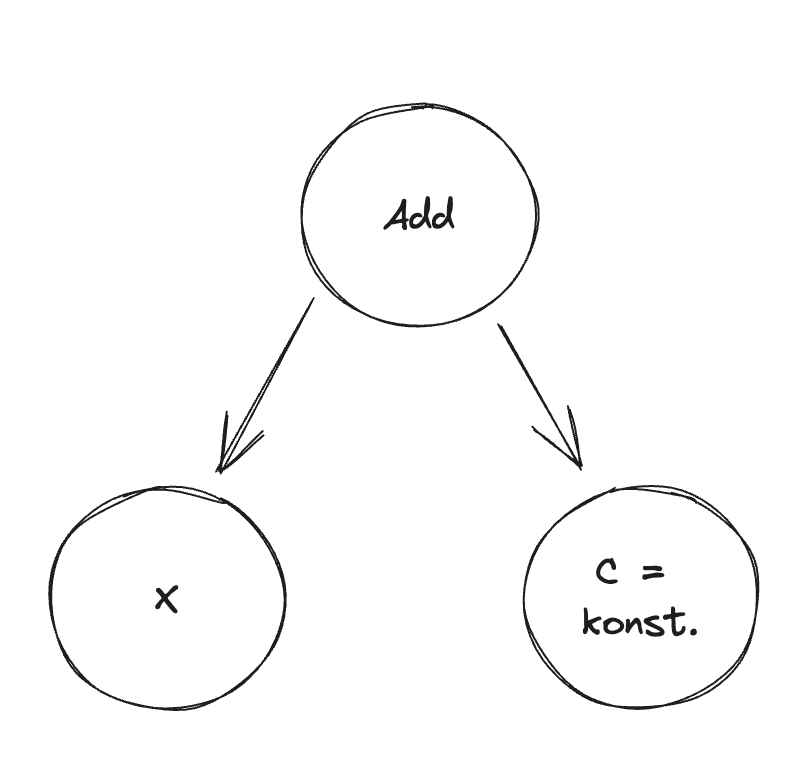
\includegraphics[width=100pt, height=100pt]{assets/start-tree.png}
          \pause
          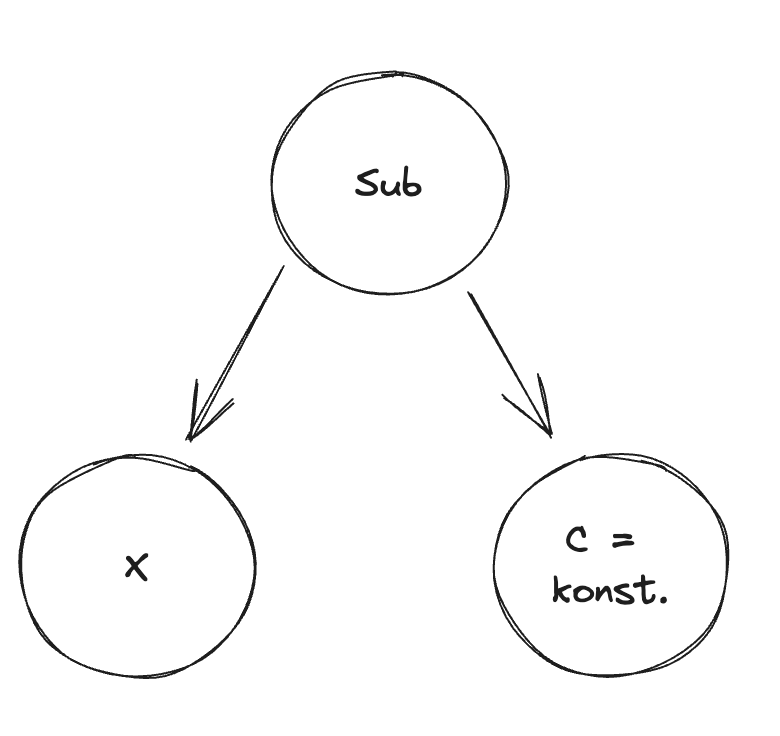
\includegraphics[width=100pt, height=100pt]{assets/start-tree-2.png}
        \end{figure}
        \pause
      \item Vůči těmto vzorům budou náhodně vygenerovány nové podstromy a proběhne ,,crossover'' 
        \pause
      \item Poté jsou vyhodnoceny korelační koeficienty obou nově vzniklých datasetů 
    \end{enumerate}
 \end{block} 
\end{frame}

\begin{frame}{Teoretická část - Algoritmus pro hledání vzorce korelace}
  \begin{block}{Pseudo-algoritmus}
    \begin{enumerate}
        \setcounter{enumi}{4}
       \item V předkovi, který získá lepší korelační koeficient se náhodně zafixuje pozice po kterou zůstane strom původní %TODO 2-point crossover?
        \item Algoritmus poté opět pokračuje bodem 2 
       \item Algoritmus skončí po pevně daném počtu iterací 
         \begin{itemize}
            \item Konkrétní počet bude stanoven empiricky
         \end{itemize}
    \end{enumerate}
 \end{block} 
\end{frame}

\begin{frame}{}
  \begin{center}
    Praktická část
  \end{center} 
\end{frame}

\begin{frame}{Praktická část}
	\begin{enumerate}
    \item Teoretická část
      \begin{itemize}
        \item Analýza zadání 
        \item Analýza související studie a dostupných dat 
        \item Normalizace dat
        \item Algoritmus pro hledání vzorce korelace
        \item Výpočet korelace dat
      \end{itemize}

    \item Praktická část
      \begin{itemize}
        \item Control a Data flow diagram
      \end{itemize}
  \end{enumerate}
\end{frame}

\begin{frame}{Praktická část}
  \begin{center}
    Control a Data flow diagram
  \end{center} 
\end{frame}

\begin{frame}{Praktická část}
	\begin{enumerate}
    \item Teoretická část
      \begin{itemize}
        \item Analýza zadání 
        \item Analýza související studie a dostupných dat 
        \item Normalizace dat
        \item Algoritmus pro hledání vzorce korelace
        \item Výpočet korelace dat
      \end{itemize}

    \item Praktická část
      \begin{itemize}
        \item Control a Data flow diagram
        \item Poznámky k řešení
      \end{itemize}
  \end{enumerate}
\end{frame}

\begin{frame}{Praktická část}
 \begin{center}
  Poznámky k řešení
 \end{center} 
\end{frame}

\begin{frame}{Praktická část}
  \begin{block}{Poznámky k řešení}
    \begin{itemize}
        \pause
      \item Veškeré hodnoty ACC a HR lze reprezentovat v rámci \textcolor{Red}{signed}, respektive \textcolor{Red}{unsigned byte}
        \pause
        \begin{itemize}
          \item Naprosto ideální pro \textcolor{Red}{vektorové} zpracování v rámci prezentovaných front/polí a optimalizace vůči \textit{cache}
        \end{itemize}
    \end{itemize} 
  \end{block}
\end{frame}

\begin{frame}{Praktická část}
	\begin{enumerate}
    \item Teoretická část
      \begin{itemize}
        \item Analýza zadání 
        \item Analýza související studie a dostupných dat 
        \item Normalizace dat
        \item Algoritmus pro hledání vzorce korelace
        \item Výpočet korelace dat
      \end{itemize}

    \item Praktická část
      \begin{itemize}
        \item Control a Data flow diagram
        \item Poznámky k řešení
      \end{itemize}
    \item Závěr
  \end{enumerate}
\end{frame}

\begin{frame}
  \begin{center}
    Závěr 
  \end{center}
\end{frame}

\begin{frame}{Závěr}
  \begin{block}{Body k zamyšlení}
    \begin{itemize}
        \pause
      \item One-point vs. K-point crossover
        \pause
      \item Zlepšení konvergence algoritmu
        \begin{itemize}
            \pause
          \item Lépe zakomponovat výsledek korelace do výběru crossover bodu 
        \end{itemize}
     \end{itemize}
  \end{block}
\end{frame}

\begin{frame}
  \begin{center}
    Děkuji Vám za pozornost! 
  \end{center}
\end{frame}


\end{document}
